\documentclass[a4paper, 11pt]{book}
\usepackage[T1]{fontenc}
\usepackage[utf8]{inputenc}
\usepackage[italian]{babel}

% ---- PACCHETTI ----
\usepackage{amsmath}
\usepackage{amsfonts}
\usepackage{amssymb}
\usepackage{amsthm}
\usepackage{physics}

\usepackage{graphicx}
\usepackage{tikz}
% \usepackage{ntheorem}
\usepackage{enumitem}
\usepackage{titlesec}

\usepackage{xurl}
\usepackage[backend=bibtex,style=numeric-comp]{biblatex}

\addbibresource{bibliography.bib}

% ---- REIMPOSTAZIONI ----
\renewcommand\thesection{\arabic{section}} % Rimuove il numero del capitolo dal numero della sezione %
\numberwithin{equation}{chapter} % Aggiunge il numero del capitolo all'equazione %
\let\MakeUppercase\relax % Rende gli header in ogni pagina (capitolo - paragrafo) NON Caps %
\DeclareEmphSequence{\bfseries}
% \titleformat{\chapter}

% ---- AMBIENTI PERSONALI ----
\newtheorem{lemma}{Lemma}[chapter]

% ---- COMANDI PERSONALI ----
\newcommand{\N}{\mathbb{N}}
\newcommand{\Z}{\mathbb{Z}}
\newcommand{\E}{\mathbb{E}}
\newcommand{\R}{\mathbb{R}}
\newcommand{\C}{\mathbb{C}}
\newcommand{\LL}{\mathcal{L}}

\newcommand{\func}[3]{#1:#2\rightarrow#3}
\newcommand{\myexp}[1]{e^{#1}}
\newcommand{\lagrange}[3]{\dv{t}\pdv{#1}{#3}-\pdv{#1}{#2}}
\newcommand{\mycomment}[1]{}

\begin{document}
\begin{titlepage}
    \begin{center}
        \begin{minipage}[ht!]{0.49\textwidth}
                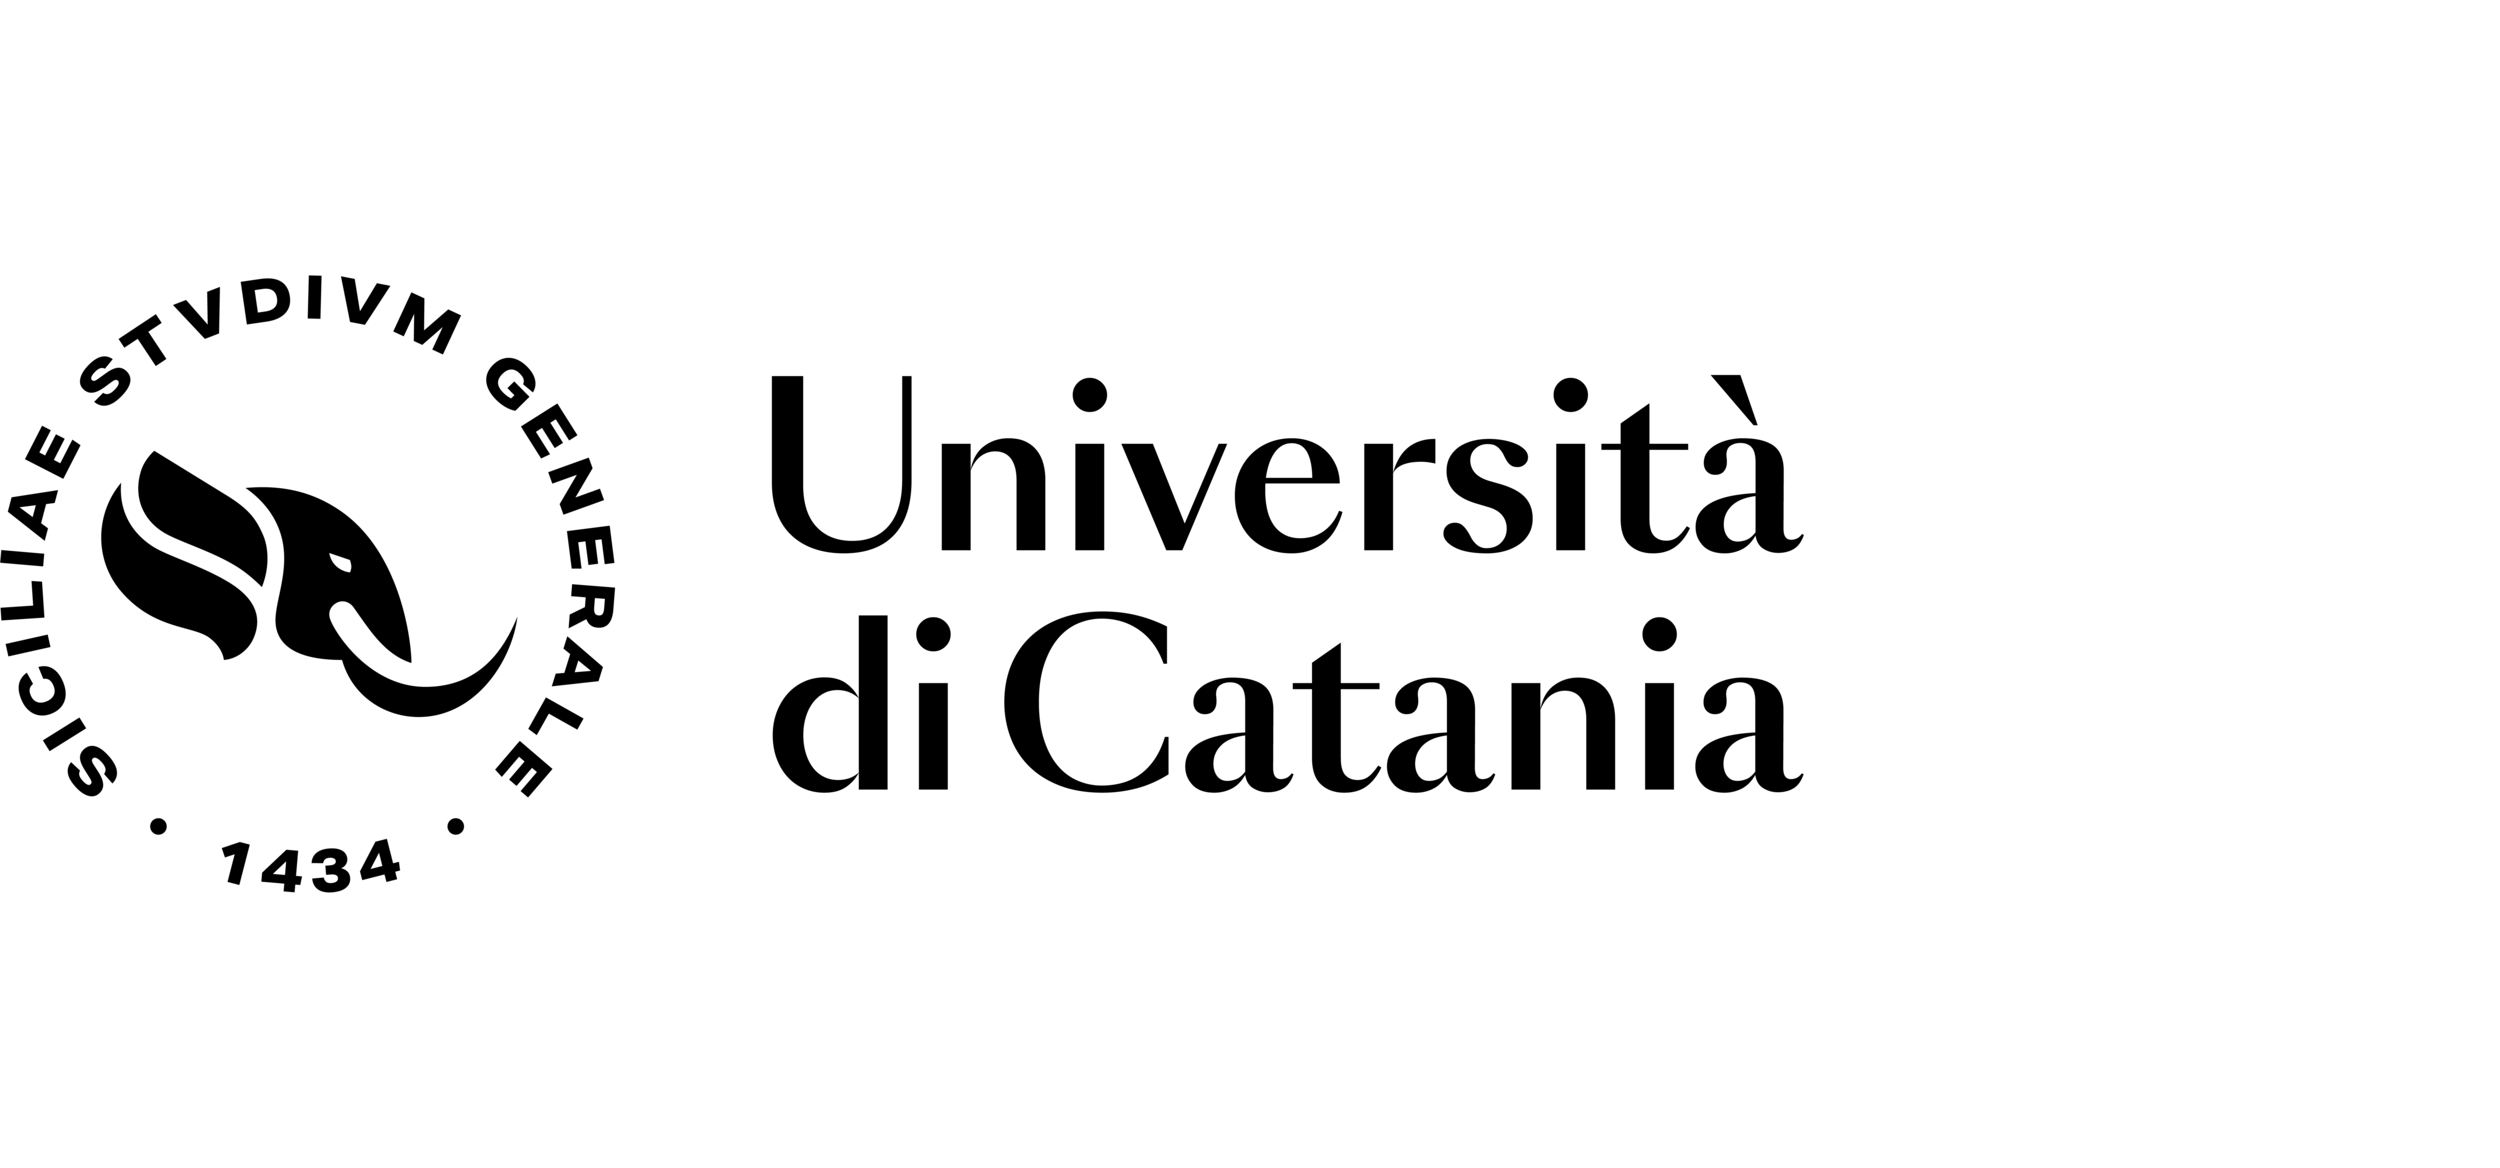
\includegraphics[width=\textwidth]{images/LogoUniCT.png}
        \end{minipage}
        \hfill
        \begin{minipage}[th!]{0.49\textwidth}
                
\includegraphics[width=\textwidth]{images/LogoDFA.png}
        \end{minipage}
        \large
        \textbf{CORSO DI LAUREA IN FISICA}
        \vspace{0.5cm}
        \hrule
        \vspace{3cm}
        
        \centering

        Appunti di\\\Huge{\textbf{OSCILLAZIONI E ONDE}}\\
        
        \vfill
        
        \begin{minipage}[h]{0.35\textwidth}
            \hrule
            \vspace{0.3cm}
            \small \centering
            Abstract
            \vspace{0.35cm}
            \hrule
        \end{minipage}
        
        \vfill
        
        \hrule
        \vspace{0.3cm}
        \normalsize
        \textbf{Anno Accademico 2023/2024}
    \end{center}
\end{titlepage}

\pagenumbering{Roman}
\chapter*{Prefazione}\label{s:preface}
[BOZZA] Ho deciso di stendere questa trascrizione in $\text{\LaTeX}$ degli appunti del corso Oscillazioni e Onde tenuto dal prof. Fabio Siringo durante l'A.A. 2023/2024 con l'intento di avere una raccolta organica e quanto pi\`u chiara possibile del materiale, vista l'attuale assenza di un libro di testo per il programma svolto. Nel corso della scrittura ho voluto prendermi la libert\`a di approfondire, ove lo ritenessi necessario ai fini della completezza e della chiarezza, con materiale preso da testi di Meccanica e di Matematica. \par Tengo particolarmente a sottolineare la natura personale degli appunti che non vogliono sostituirsi alle lezioni tenute dal docente o ai libri di testo, tuttavia invito chiunque lo ritenesse utile a farne un libero uso con la consapevolezza di quanto appena detto. A tal proposito, in caso il lettore dovesse riscontrare errori o volesse suggerire delle modifiche, \`e pregato di contattarmi presso:
\begin{verbatim}
    pappalardoaurelio@gmail.com
\end{verbatim}\par
Al seguente link è possibile accedere alla versione più aggiornata degli appunti: 

\begin{center}
    Ultima modifica: \today
\end{center}

% INSERIRE LINK
\chapter*{Programma del Corso}
[BOZZA] Ciao, qui andrà il programma
\begin{titlepage}
    \tableofcontents
\end{titlepage}

\pagenumbering{arabic}
% - % - % - % - % - % - % - % - % - % - % - % - %
%  ______   ______        _____     ______      %
% /\__  _\ /\  __ \      /\  __-.  /\  __ \     %
% \/_/\ \/ \ \ \/\ \     \ \ \/\ \ \ \ \/\ \    %
%    \ \_\  \ \_____\     \ \____-  \ \_____\   %
%     \/_/   \/_____/      \/____/   \/_____/   %
% - % - % - % - % - % - % - % - % - % - % - % - %
% [ ] Sistemare introduzione (copiare il Goldstein!!! \eta^\alpha idea molto bella)
% [ ] Label capitolo
% [ ] Reference appendice
% [ ] Caso Anisotropo più compatto
% [ ] Finire caso 3D!!!
% [ ] Laurearsi
% [ ] Spazio di Bruillon?
% [ ] Relazione di dispersione?
% [x] Spezzare il calcolo diagon. pot. per N molle (sviluppare \zeta_n^2 a parte e poi mettere nella sommatoria)
\chapter{L'Oscillatore Armonico}
    \section{Introduzione}
    Dato un sistema fisico le cui configurazioni sono identificate dalle coordinate pure $q^\alpha$, dalla meccanica \`e noto che le configurazioni di equilibrio stabile si hanno in corrispondenza dei minimi del potenziale $V\qty(q^\alpha)$. Assumendo che $V$ sia una funzione almeno di classe $C^2$ e che ammetta minimo, \`e possibile effettuare una traslazione che ponga l'origine del S.d.R.\footnote{Sistema di riferimento} coincidente col punto di minimo e sviluppare in serie di Taylor/Mac Laurin il potenziale, arrestandosi al termine di secondo grado. Si ottiene dunque: $$V\qty(q^\alpha)=V\qty(\vb{0})+\pdv{V}{q^\alpha}\eval_{\vb{0}}q^\alpha+\frac{1}{2}\pdv{V}{q^\alpha}{q^\beta}\eval_{\vb{0}}q^\alpha q^\beta+R\qty(q^\alpha).$$ Ricordando che il potenziale \`e definito a meno di una costante additiva e che all'equilibrio $\displaystyle\pdv{V}{q^\alpha}\eval_{\vb{0}}=0$, e trascurando il termine infinitesimo, si pu\`o riscrivere il potenziale come\cite{Goldstein2005-jd}:
    \begin{equation}
        V\qty(q^\alpha)=\frac{1}{2}\pdv{V}{q^\alpha}{q^\beta}\eval_{\vb{0}}q^\alpha q^\beta,
        \label{eq:potenziale:1}
    \end{equation} che non \`e altro che una forma quadratica del tipo $\displaystyle\frac{1}{2}\qty[\underline{x}^\top H_V\qty(\vb{0})\underline{x}]$, con $\underline{x}\in\R^n$ un punto e $H_V\qty(\vb{0})$ la matrice Hessiana di $V$ calcolata in $\vb{0}$. \par Ovviamente questo \`e soltanto un modello approssimato che pu\`o essere applicato in un intorno del minimo. Se ci si allontana troppo, le discordanze tra il modello e le misure che si riscontrano prendono il nome di \emph{effetti anarmonici}.
\section{Oscillatore Armonico Unidimensionale}
    Applichiamo quanto detto al caso unidimensionale. Siano $A\subseteq\R$ un aperto, $\func{V}{A}{\R}$ una funzione di classe $C^2$ e $x_0\in A$ un punto di minimo per $V$. La \eqref{eq:potenziale:1} diventa: $$V(x-x_0)=\frac{1}{2}\dv[2]{V}{x}\eval_{x_0}\qty(x-x_0)^2;$$ ponendo $u=x-x_0$, si effettua la traslazione che pone il punto di minimo nell'origine, per cui si ottiene: $$V(u)=\frac{1}{2}\dv[2]{V}{x}\eval_{0}u^2.$$ \par A questo punto risulta evidente la somiglianza con il potenziale della forza elastica. Ponendo $\displaystyle k=\dv[2]{V}{x}\eval_{x_0}$ e prendendone il "gradiente" (derivata prima) cambiato di segno, si ottiene l'espressione della forza elastica tramite la legge di Hooke: $$V\qty(u)=\frac{1}{2}ku^2 \implies \vb{F\qty(\vb{u})}=-\dv{V}{x}\vu{i}=-k\vb{u},$$ da cui l'equazione del moto: $m\ddot{u}=-ku$, che \`e lineare omogenea del secondo ordine. \par Ponendo $\frac{k}{m}=\omega^2$, si pu\`o scrivere $\ddot{u}=-\omega^2u$, di cui due soluzioni linearmente indipendenti sono $\cos\qty(\omega t)$ e $\sin\qty(\omega t)$. L'integrale generale \`e quindi $$u\qty(t)=c_1\cos\qty(\omega t)+c_2\sin\qty(\omega t)$$ con $c_1,c_2\in\R$, o alternativamente, ponendo $c_1=A\cos\phi$ e $c_2=-A\sin\phi$, ancora con $A,\phi\in\R$, $$u\qty(t)=A\cos\qty(\omega t+\phi).$$ In tal caso, $A$ si dice \emph{ampiezza}, $\omega$ si dice \emph{pulsazione} o \emph{frequenza angolare} e $\omega t+\phi$ si dice \emph{fase}.
\section{Oscillatore Armonico Bidimensionale}
    Proviamo ora passo passo ad aumentare il numero di dimensioni, per semplicit\`a iniziamo da 2. Quando vi \`e pi\`u di un grado di libert\`a, \`e importante distinguere i casi in base alle simmetrie che il sistema presenta. Se il potenziale \`e invariante per rotazioni, diciamo che l'oscillatore armonico \`e \emph{isotropo}, altrimenti lo diciamo \emph{anisotropo}.
    \subsection{Oscillatore isotropo}
        Come prima, supponiamo di avere $\func{V}{A\subseteq{\R^2}}{\R}$, definito dalla legge: $$V\qty(x,y)=\frac{1}{2}m\omega^2\qty(x^2+y^2),$$ ove si \`e usata la relazione $k=m\omega^2$. Notiamo subito che il potenziale \`e invariante per rotazioni in quanto le curve equipotenziali sono circonferenze centrate nell'origine\footnote{Immaginiamo di trovarci gi\`a nel sistema di riferimento scelto in modo da collocare un punto di minimo di $V$ nell'origine, se cos\`i non fossoe, \`e sempre possibile ricondursi a quel caso con una traslazione}. Di conseguenza $V$ si spezza facilmente in: $$V\qty(x,y)=\frac{1}{2}m\omega^2x^2+\frac{1}{2}m\omega^2y^2$$ e derivando si ottengono quindi le due equazioni del moto gi\`a disaccoppiate.
        \begin{equation*}
        \begin{cases}
            \ddot{x}=-\omega^2x\\
            \ddot{y}=-\omega^2y
        \end{cases}
        \end{equation*}
        le cui soluzioni sono nuovamente le funzioni $x\qty(t)=A_1\cos(\omega t+\phi_1)$ e $y\qty(t)=A_2\cos(\omega t+\phi_2)$, definite a meno di quattro costanti arbitrarie. Fissando le condizioni iniziali: $x\qty(0)$, $\dot{x}\qty(0)$, $y\qty(0)$ e $\dot{y}\qty(0)$, \`e possibile trovare l'unica soluzione del problema di Cauchy.
    \subsection{Oscillatore anisotropo}
        Affrontiamo adesso il caso di un potenziale che non presenti simmetrie per rotazione, ad esempio: $$V\qty(x,y)=\frac{1}{2}m\omega^2x^2+\frac{1}{2}m\omega^2y^2+2\gamma xy,\quad\gamma>0.$$
        \subsubsection{Diagonalizzazione del potenziale}
            Come \`e noto dalla \eqref{eq:potenziale:1}, \`e possibile riscrivere il potenziale come forma quadratica: $$\frac{1}{2}m\omega^2\mqty(x&y)\mqty[1 & \frac{\gamma}{m\omega^2} \\ \frac{\gamma}{m\omega^2} & 1]\mqty(x\\y).$$ Poich\`e la matrice dei coefficienti \`e simmetrica, per il teorema spettrale \`e diagonalizzabile ed esiste quindi un cambio di coordinate che pone la forma quadratica in forma canonica, disaccoppiando di conseguenza le equazioni del moto. \par Le nuove coordinate sono quelle identificate da una base (ortonormale) di autovettori della matrice, cerchiamo quindi gli zeri del polinomio caratteristico: $$P\qty(\lambda)=\det\mqty[1-\lambda & \frac{\gamma}{m\omega^2} \\ \frac{\gamma}{m\omega^2} & 1-\lambda]=\qty(1-\lambda)^2-\frac{\gamma^2}{m^2\omega^4}=0\implies\lambda_{\pm}=1\pm\frac{\gamma}{m\omega^2}.$$ Calcoliamo ora gli autovettori\footnote{O meglio, le loro componenti rispetto alla base canonica di $\R^2$: $\qty{e_1,e_2}$} $Q_{\pm}$ associati agli autovalori $\lambda_{\pm}$, risolvendo i due sistemi:
            \begin{equation*}
            \begin{cases}
                \displaystyle\qty(1-\lambda_{\pm})x+\frac{\gamma}{m\omega^2}y=0\\\\
                \displaystyle\qty(1-\lambda_{\pm})y+\frac{\gamma}{m\omega^2}x=0
            \end{cases}
            \end{equation*}
            e ottenendo quindi le componenti degli autovettori, $\qty[Q_{\pm}]=[x,\pm x]$. Scegliamo quindi due autovettori normalizzati: $$Q_{+}=\frac{1}{\sqrt{2}}\mqty(1 \\ -1),\quad Q_{-}=\frac{1}{\sqrt{2}}\mqty(1 \\ 1)$$ e la conseguente matrice di rotazione $$P=\frac{1}{\sqrt{2}}\mqty[1 & 1 \\ -1 & 1]\quad\text{tale che}\quad\mqty[1-\frac{\gamma}{m\omega^2} & 0 \\ 0 & 1+\frac{\gamma}{m\omega^2}]=P^\top\mqty[1 & \frac{\gamma}{m\omega^2} \\ \frac{\gamma}{m\omega^2} & 1]P.$$ Troviamo ora $e_1$ ed $e_2$ nelle nuove coordinate tramite i due sistemi vettoriali:
            \begin{align*}
                e_1=xQ_++yQ_- & \iff \mqty(1 \\ 0)=\frac{1}{\sqrt{2}}\qty[x\mqty(1 \\ -1)+y\mqty(1 \\ 1)] \\\\
                e_2=xQ_++yQ_- & \iff \mqty(0 \\ 1)=\frac{1}{\sqrt{2}}\qty[x\mqty(1 \\ -1)+y\mqty(1 \\ 1)] 
            \end{align*}
            da cui $e_1=\frac{1}{\sqrt{2}}\qty(Q_++Q_-)$, $e_2=\frac{1}{\sqrt{2}}\qty(Q_+-Q_-)$. Trasformando le coordinate si ottiene il nuovo potenziale: $$V\qty(Q_+,Q_-)=\frac{1}{2}m\omega^2\qty(Q_+^2+Q_-^2)+\frac{\gamma}{2}\qty(Q_+^2-Q_-^2),$$ che si spezza facilmente in: $$V\qty(Q_+,Q_-)=\frac{1}{2}m\Omega_+^2Q_+^2+\frac{1}{2}m\Omega_-^2Q_-^2,$$ avendo fatto la posizione $\Omega_\pm^2=\omega^2\qty(1\pm\frac{\gamma}{m\omega^2})$.
        \subsubsection{Equazioni del moto}
            A questo punto trovare e risolvere le equazioni del moto \`e banale: $$\ddot{Q}_\pm=-\Omega_\pm^2Q_\pm \implies Q_\pm\qty(t)=A_\pm\cos\qty(\Omega_\pm t+\phi_\pm),$$ e attraverso la trasformazione inversa \`e possibile ricavare le $x\qty(t)$, $y\qty(t)$:
            \begin{align*}
                & x\qty(t)=\frac{Q_+\qty(t)+Q_-\qty(t)}{\sqrt{2}}=\frac{1}{\sqrt{2}}\qty[A_+\cos\qty(\Omega_+t+\phi_+)+A_-\cos\qty(\Omega_-t+\phi_-)] \\
                & y\qty(t)=\frac{Q_+\qty(t)-Q_-\qty(t)}{\sqrt{2}}=\frac{1}{\sqrt{2}}\qty[A_+\cos\qty(\Omega_+t+\phi_+)-A_-\cos\qty(\Omega_-t+\phi_-)]
            \end{align*}
            Dove, come ci aspettavamo, $A_\pm$ e $\phi_\pm$ sono quattro costanti reali determinabili conoscendo le condizioni iniziali.
        \subsubsection{Energia cinetica}
            Avendo operato una rotazione che non altera la metrica, ci aspettiamo che l'energia cinetica $T$ resti invariata da un S.d.R. all'altro. \par Dalla definizione $\displaystyle T=\frac{1}{2}m\norm{\vb{v}}^2$, sviluppando il prodotto scalare otteniamo: $$T=\frac{1}{2}m\qty(\dot{x}^2+\dot{y}^2)$$ Derivando le equazioni di trasformazione invece troviamo:
            \begin{align*}
                &\dv{x}{t}=\dv{t}\frac{Q_++Q_-}{\sqrt{2}}=\frac{\dot{Q}_++\dot{Q}_-}{\sqrt{2}}\\
                &\dv{y}{t}=\dv{t}\frac{Q_+-Q_-}{\sqrt{2}}=\frac{\dot{Q}_+-\dot{Q}_-}{\sqrt{2}}
            \end{align*}
            e sostituendo nell'energia cinetica: $$T=\frac{1}{2}m\qty[\frac{\qty(\dot{Q}_++\dot{Q}_-)^2}{2}+\frac{\qty(\dot{Q}_++\dot{Q}_-)^2}{2}]=\frac{1}{2}m\qty(\dot{Q}_+^2+\dot{Q}_-^2),$$ che prova quanto affermato.
\section{Oscillatore a tre Gradi di Libert\`a}
    Proviamo ora a generalizzare ulteriormente quanto detto fin'ora per sistemi che abbiano pi\`u di due gradi di libert\`a. Iniziamo considerando il caso di tre masse legate da molle ideali con estremi liberi, per poi affrontare il caso con condizioni armoniche al contorno e successivamente generalizzare a $n$ masse.
    \subsection{Tre masse a estremi liberi}
        Prendiamo in esame un sistema fisico formato da tre masse uguali $m$ vincolate a muoversi sull'asse $x$, collegate da due molle di costante $k=m\omega^2$. \par Le configurazioni di questo sistema fisico sono identificate dalle coordinate generalizzate $q^\alpha=\qty{x,y,z}$ che indicano la posizione delle tre massse rispetto all'origine. Sul sistema agiscono due forze, entrambe forze elastiche, che dipendono dalle due distanze $\qty(y-x)$ e $\qty(z-y)$. Possiamo facilmente calcolare il potenziale elastico delle molle: $$V\qty(x,y,z)=\frac{1}{2}m\omega^2\qty(x-y)^2+\frac{1}{2}m\omega^2\qty(y-z)^2=$$ $$=\frac{1}{2}m\omega^2\qty(x^2-2xy+2y^2-2yz+z^2),$$ la cui matrice associata \`e $\displaystyle B=\mqty[1 & -1 & 0 \\ -1 & 2 & -1 \\ 0 & -1 & 1]$. Procediamo come precedentemente per diagonalizzare il potenziale: $$P\qty(\lambda)=\det\mqty[1-\lambda & -1 & 0 \\ -1 & 2-\lambda & -1 \\ 0 & -1 & 1-\lambda]=\lambda\qty(1-\lambda)\qty(\lambda-3).$$ Gli autovalori sono $\lambda_0=0$, $\lambda_1=1$ e $\lambda_3=3$. Dal calcolo degli autovettori associati otteniamo le componenti dei vettori normalizzati $$q_0=\frac{1}{\sqrt{3}}\mqty(1 \\ 1 \\ 1),\quad q_1=\frac{1}{\sqrt{2}}\mqty(1 \\ 0 \\ -1),\quad q_3=\frac{1}{\sqrt{6}}\mqty(1 \\ -2 \\ 1),$$ con cui possiamo costruire la matrice di rotazione $P$ tale che $\det P=1$ contenente $q_3$, $q_1$ e $q_0$ sulle colonne, che diagonalizza il potenziale: $$D=P^\top BP \iff PDP^\top=B.$$ Sostituendo $B$ nella forma quadratica: $$V\qty(x,y,z)=\frac{1}{2}m\omega^2\mqty(x & y & z)PBP^\top\mqty(x\\y\\z),$$ dove, come prima \`e stato mostrato in maniera pi\`u esplicita, $P^\top\mqty(x\\y\\z)$ trasforma le coordinate, il potenziale assume la forma: $$V(q_3,q_1,q_0)=\frac{1}{2}m\omega^2\mqty(q_3 & q_1 & q_0)\mqty[\dmat[0]{3,1,0}]\mqty(q_3 \\ q_1 \\ q_0)=\frac{1}{2}m\omega^2\qty(3q_3^2+q_1^2)$$ e, ponendo di nuovo $\Omega_3^2=3\omega^2$ e $\Omega_1^2=\omega^2$, otteniamo le equazioni del moto:
        \begin{equation*}
        \begin{cases}
            \ddot{q}_0=0\\
            \ddot{q}_1=-\Omega_1^2q_1\\
            \ddot{q}_3=-\Omega_3^2q_3
        \end{cases}
        \iff
        \begin{cases}
            q_0\qty(t)=v_0t+s_0\\
            q_1\qty(t)=A_1\cos\qty(\Omega_1 t+\phi_1)\\
            q_3\qty(t)=A_3\cos\qty(\Omega_3 t+\phi_3)
        \end{cases}
        \end{equation*}
        Applicando la trasformazione di coordinate inversa data da $\mqty(x \\ y \\ z)=P\mqty(q_3 \\ q_1 \\ q_0)$ possiamo trovare $x\qty(t)$, $y\qty(t)$ e $z\qty(t)$:
        \begin{align*}
            &x\qty(t)=\frac{1}{\sqrt{3}}\qty(v_0t+s_0)+\frac{A_1}{\sqrt{2}}\cos\qty(\Omega_1t+\phi_1)+\frac{A_3}{\sqrt{6}}\cos\qty(\Omega_3t+\phi_3)\\
            &y\qty(t)=\frac{1}{\sqrt{3}}\qty(v_0t+s_0)-\frac{2A_3}{\sqrt{6}}\cos\qty(\Omega_3t+\phi_3)\\
            &z\qty(t)=\frac{1}{\sqrt{3}}\qty(v_0t+s_0)-\frac{A_1}{\sqrt{2}}\cos\qty(\Omega_1t+\phi_1)+\frac{A_3}{\sqrt{3}}\cos\qty(\Omega_3t+\phi_3)
        \end{align*}
        Come ci potevamo aspettare dalla presenza di tre equazioni lineari del secondo ordine, le equazioni del moto sono definite a meno di sei costanti arbitrarie: $v_0$, $s_0$, $A_1$, $\phi_1$, $A_3$ e $\phi_3$. \`E inoltre importante sottolineare il significato fisico legato alla presenza di $\lambda_0=0$ tra gli autovalori: possiamo notare che l'equazione del moto associata alla coordinata $q_0$ costituisce un moto rettilineo uniforme, e non oscillatorio, che suggerisce una simmetria del sistema per traslazioni. \par A questo punto risulta utile introdurre il concetto di \emph{modi normali di oscillazione}.
    \subsection{Tre masse con condizioni periodiche al contorno}
        Supponiamo adesso di avere tre masse disposte come nell'esempio precedente ma con l'ulteriore condizione che la prima e la terza massa interagiscano per mezzo di una terza molla di caratteristiche uguali alle altre due. Questa situazione fisica pu\`o essere meglio visualizzata come se sia le masse che le molle fossero vincolate a scorrere su di una circonferenza rigida $\gamma$ priva di attrito. \par Anche in questo caso possiamo ricorrere alle coordinate pure $x$, $y$ e $z$ che stavolta rappresentano le ascisse curvilinee condotte da un arbitraio punto $O\in\gamma$ fino a individuare la posizione delle tre masse. Il potenziale, similmente a prima, si presenta come: 
        \begin{multline*}
            V=\frac{1}{2}\omega^2\qty[\qty(x-y)^2+\qty(y-z)^2+\qty(z-x)^2]=\\=\frac{1}{2}m\omega^2\mqty(x & y & z)\mqty[\dmat[-1]{2,2,2}]\mqty(x \\ y \\ z)=\frac{1}{2}m\omega^2\underline{x}^\top B\underline{x}.
        \end{multline*}
        Eseguiamo il solito procedimento per diagonalizzare $B$: $$P\qty(\lambda)=\det\mqty[\dmat[-1]{2-\lambda,2-\lambda,2-\lambda}]=-\lambda\qty(\lambda-3)^2=0,$$ che d\`a gli autovalori $\lambda_0=0$ e $\lambda_3=3$ doppio. Gli autovettori normalizzati che se ne ricavano sono: $$q_0=\frac{1}{\sqrt{3}}\mqty(1 & 1 & 1)\quad q_{3,1}=\frac{1}{\sqrt{}}\mqty( & & )$$
\section{Oscillatore a $N$ Gradi di Libert\`a}
    Generalizziamo definitivamente il problema considerando il caso di una catena di $N$ masse collegate a due a due da molle di costante elastica $k=m\omega^2$ con condizioni periodiche al contorno. \par Supponiamo per comodit\`a $N$ pari, denotiamo con $a$ il passo reticolare, con $x_n=na$ la posizione di equilibrio dell'$n$-esima massa $\qty(n=0,\dots,N-1)$ e con $L=Na$ la lunghezza della catena. Siano inoltre le funzioni $\zeta_n$ la dislocazione dell'$n$-esima massa dalla posizione di equilibrio $x_n$. Richiedere che le condizioni al contorno siano periodiche vuol dire supporre che l'ultima massa possa interagire con la prima, come se la catena formasse un cerchio. In termini matematici questo si traduce in:
    \begin{align}
        &x_{n+N}=x_n+L\equiv x_n \label{eq:period:1}\\
        &\zeta_{n+N}\equiv \zeta_n \label{eq:period:2}
    \end{align} \par
    Il potenziale di un tale sistema ha forma:
    \begin{equation}
        V=\frac{1}{2}m\omega^2\sum_n\qty(\zeta_{n+1}-\zeta_n)^2.
        \label{eq:potenziale:2}
    \end{equation}
    \subsection{Ricerca dei modi normali di oscillazione}
        A questo punto desideriamo provare che le seguenti relazioni costituiscono il cambio di coordinate che permette di passare dalle $\zeta_n$ alle $Q_q$ ove il potenziale \`e diagonalizzato:
        \begin{align}
            &\zeta_n=\frac{1}{\sqrt{N}}\sum_q e^{iqx_n}Q_q \label{eq:cambio:1}\\
            &Q_q=\frac{1}{\sqrt{N}}\sum_n e^{-iqx_n}\zeta_n \label{eq:cambio:2}
        \end{align}
        Allo scopo di dileguare eventuali perplessit\`a, vorrei giustificare rapidamente la presenza di esponenziali complessi nelle relazioni appena enunciate. Ci si potrebbe aspettare infatti, che le trasformazioni da cercare siano simili a quelle viste nei casi semplificati a due e tre dimensioni: somme di funzioni trigonometriche con opportuni coefficienti. Volendo, potremmo affrontare questo problema proprio in questo modo, se non fosse che ci\`o renderebbe i calcoli ben pi\`u tediosi, quando invece operare con gli esponenziali complessi elimina questo problema. Infatti, basta tenere a mente che $e^{i\theta}=\cos\theta+i\sin\theta$ e che di consguenza ci baster\`a prendere la parte reale della soluzione per raggiungere il nostro obiettivo. Sostanzialmente stiamo affrontando un problema di moto armonico in $\R$ risolvendo il corrispettivo problema di `moto circolare' in $\C$ e `proiettandolo' su $\R$. Si rimanda all'appendice A per qualche cenno in pi\`u ai numeri complessi.
                                    %%%%%%%%%%%%%%%%%%%%%%%%%%%%%%%%%%%%%%%%%%%%%%%%%%%%%%%%%
                                    % ATTENZIONE!!! Togliere "Appendice A" e usare un Label %
                                    %%%%%%%%%%%%%%%%%%%%%%%%%%%%%%%%%%%%%%%%%%%%%%%%%%%%%%%%%
        \par Osserviamo subito che da \eqref{eq:period:1} e \eqref{eq:cambio:1} \`e possibile conoscere l'intervallo in cui variano le $q$: $$e^{iqx_{n+N}}=e^{iqx_n} \iff e^{iqna}e^{iqL}=e^{iqna} \iff e^{iqL}=1,$$ per cui deve essere $qL=2m\pi$, con $m\in\Z$. Sostituendo $L$ otteniamo:
        \begin{equation}
            q=\frac{2m\pi}{L}=\frac{2\pi}{a}\frac{m}{N}
            \label{eq:q}
        \end{equation}
        Dal momento che i gradi di libert\`a sono $N$, prevediamo che siano presenti proprio $N$ modi normali al variare di $q$, per cui possiamo scegliere $N$ diversi valori di $q$ al variare di $m\in\Z$. Risulta opportuna la scelta di un intervallo simmetrico $\displaystyle m\in\left[-\frac{N}{2};\frac{N}{2}\right[$, in modo che si abbia $\displaystyle q\in\left[-\frac{\pi}{a};\frac{\pi}{a}\right[$. Per compattezza della notazione, questo fatto sar\`a omesso nella scrittura degli indici della sommatoria laddove ci\`o non possa causare ambiguit\`a. 
        \par Prima di proseguire oltre con la risoluzione del problema, anteponiamo dei risultati utili:
        \begin{lemma} \label{lm:delta}
            Sotto le ipotesi del problema valgono le seguenti relazioni:
            \begin{align}
                &\sum_{n}e^{iqx_n}=N\delta_{q,0} &n=0,\dots,N-1 \label{eq:delta:1}\\
                &\sum_{q}e^{-iqx_n}=N\delta_{n,0} &q\in\left[-\frac{\pi}{a};\frac{\pi}{a}\right[ \label{eq:delta:2}
            \end{align}
        ove $\delta_{\alpha,\beta}$ \`e la Delta di Kronecker.
        \end{lemma}
        \begin{proof}
            Proviamo la \eqref{eq:delta:1}. \par Se $q=0$, banalmente: $$\sum_{n=0}^{N-1}1=N.$$ \par Se $q\neq0$, osserviamo che si pu\`o scrivere: $$\sum_{n=0}^{N-1} e^{iqx_n}=\sum_{n=0}^{N-1} e^{iqna}=\sum_{n=0}^{N-1}\qty(e^{iqa})^n=\frac{1-e^{iqNa}}{1-e^{iqa}}$$ essendo il termine generale della successione delle somme parziali di una serie geometrica di ragione $e^{iqa}$. Sostituendo la \eqref{eq:q} si vede subito che tale somma risulta $0$. \\ Allo stesso modo si prova la \eqref{eq:delta:2}.
        \end{proof}
        \par Verifichiamo adesso che le trasformazioni \eqref{eq:cambio:1} e \eqref{eq:cambio:2} sono l'una l'inversa dell'altra mostrando che la loro composizione restituisce l'identit\`a: $$\zeta_n=\frac{1}{\sqrt{N}}\sum_{q}e^{iqx_n}\qty(\frac{1}{\sqrt{N}}\sum_{p=0}^e{N-1}e^{-iqx_p}\zeta_p)=\frac{1}{N}\sum_{p,q}e^{iq\qty(x_n-x_p)}\zeta_p.$$ Poich\'e $\zeta_p$ non dipende da $q$, \`e possibile estrarlo dalla rispettiva sommatoria: $$\zeta_n=\frac{1}{N}\sum_p\zeta_p\qty[\sum_q e^{iq\qty(x_n-x_p)}]$$ dove per il Lemma \ref{lm:delta} si pu\`o scrivere: $$\zeta_n=\frac{1}{N}\sum_p\zeta_p\delta_{n,p}=\zeta_n$$ che \`e appunto l'identit\`a. \par Ci chiediamo quindi se questo cambio di coordinate ci fornisca i modi normali di oscillazione del sistema, diagonalizzando \eqref{eq:potenziale:2}. Studiamo la seguente quantit\`a:
        \begin{multline*}
            \zeta_n^2=\frac{1}{N}\qty(\sum_q e^{iqx_n}Q_q)^2=\frac{1}{N}\qty(\sum_q e^{iqx_n}Q_q)\Biggl(\sum_{q'} e^{iq'x_n}Q_{q'}\Biggr)=\\=\frac{1}{N}\sum_{q,q'}Q_qQ_{q'}e^{i\qty(q+q')x_n},
        \end{multline*}
        sommiamo quindi su $n$ e applichiamo ancora il Lemma \ref{lm:delta} dopo aver raccolto i termini comuni: $$\sum_n\zeta_n^2=\frac{1}{N}\sum_{q,q'}Q_qQ_{q'}\sum_ne^{i\qty(q+q')x_n}=\frac{1}{N}\sum_{q,q'}Q_qQ_{q'}N\delta_{q,-q'}=\sum_qQ_qQ_{-q}.$$
        \par Prima di proseguire ulteriormente, facciamo delle considerazioni utili. Ricordiamo che le $\zeta_n$ sono funzioni reali e quindi deve essere $\zeta_n^*=\zeta_n$.\footnote{Con $\zeta_n^*$ indichiamo il complesso coniugato di $\zeta_n$} Inoltre, dalla \eqref{eq:cambio:1}, possiamo ricavare che $\zeta_n^*$ ha forma: $$\zeta_n^*=\frac{1}{\sqrt{N}}\sum_qe^{iqx_n}Q_q^*=\frac{1}{\sqrt{N}}\sum_{-q}e^{iqx_n}Q_{-q}^*,$$ dove, nello scrivere la seconda uguaglianza, \`e stato sfruttato il fatto che l'indice $q$ \`e saturato e quindi nulla vieta di `cambiargli il nome' in $-q$. Segue naturalmente:
        \begin{equation}
            \zeta_n=\zeta_n^* \iff Q_q=Q_{-q}^* \iff Q_{-q}=Q_q^*.
            \label{eq:QQ}
        \end{equation}
        Supponendo $Q=\alpha\qty(q)+i\beta\qty(q)$ e sostituendo quanto trovato nei conti precedenti si ottiene:
        \begin{equation}
            \sum_n\zeta_n^2=\sum_qQ_qQ_q^*=\sum_q\qty[\alpha^2\qty(q)+\beta^2\qty(q)]
            \label{eq:sommazetaquadro}
        \end{equation}
        \par A questo punto possiamo scrivere per esteso il potenziale, richiamando la \eqref{eq:potenziale:2}: $$V=\frac{1}{2}m\omega^2\sum_n\qty(\zeta_{n+1}-\zeta_n)^2$$ Valutiamo la quantit\`a tra parentesi: $$\zeta_{n+1}-\zeta_n=\frac{1}{\sqrt{N}}\sum_qQ_q\qty(e^{iqx_{n+1}}-e^{iqx_n})=\frac{1}{\sqrt{N}}\sum_qQ_qe^{iqx_n}\qty(e^{iqa}-1)$$ e inseriamola nel potenziale $V$ che, una volta sviluppato il quadrato similmente a prima e applicata la \eqref{eq:QQ}, diventa:
        \begin{multline*}
            V=\frac{1}{2}\frac{m\omega^2}{N}\sum_n\sum_{q,q'}e^{iqx_n}\qty(e^{iqa}-1)e^{iq'x_n}\bigl(e^{iq'a}-1\bigr)Q_qQ_{q'}=\\=\frac{1}{2}m\omega^2\sum_{q,q'}\delta{q,-q'}\qty(e^{iqa}-1)\bigl(e^{iq'a}-1\bigr)Q_qQ_{q'}=\\=\frac{1}{2}m\omega^2\sum_q\qty(e^{iqa}-1)\qty(e^{-iqa}-1)Q_qQ_{-q}=\\=\frac{1}{2}m\omega^2\sum_q\qty(e^{iqa}-1)\qty(e^{-iqa}-1)Q_qQ_q^*
        \end{multline*}
        Da cui l'espressione pi\`u sintetica ed elegante del potenziale:
        \begin{equation}
            V=\frac{1}{2}m\omega^2\sum_q\qty(e^{iqa}-1)\qty(e^{-iqa}-1)\norm{Q_q}^2
        \end{equation}
        che non \`e altro che una forma quadratica nelle variabili $Q_q$ la cui matrice dei coefficienti \`e diagonale e contiene gli autovalori $\qty(e^{iqa}-1)\qty(e^{-iqa}-1)$, ciascuno associato all'autovettore $Q_q$ corrispondente. Chiamiamo i vettori di base di queste nuove coordinate, $Q_q$, \emph{modi normali di oscillazione} del sistema. Queste coordinate in cui il potenziale \`e diagonale costuituiscono diversi `modi' di oscillare del sistema fisico, ciascuno linearmente indipendente dagli altri. Conseguenza di ci\`o \`e che qualunque moto periodico del sistema pu\`o essere espresso come combinazione lineare dei modi normali.
    \subsection{Risoluzione delle equazioni del moto}
        Per semplificare la forma del potenziale, moltiplichiamo e dividiamo il risultato ottenuto per $\displaystyle 4i^2e^{i\frac{qa}{2}}$. Applicando le formule di Eulero otteniamo: $$V=\frac{-4}{2}m\omega^2\sum_q\frac{e^{i\frac{qa}{2}}-e^{-i\frac{qa}{2}}}{2i}\frac{e^{-i\frac{qa}{2}}-e^{i\frac{qa}{2}}}{2i}\norm{Q_q}^2=2m\omega^2\sin^2\qty(\frac{qa}{2})\norm{Q_q}^2$$ da cui le $N$ equazioni del moto: $$-\pdv{V}{Q_q}=m\ddot{Q}_q \iff \ddot{Q}_q=4\omega^2\sin^2\qty(\frac{qa}{2})Q_q=-\Omega_q^2Q_q,$$ ponendo $\displaystyle\Omega_q=2\omega\sin\qty(\frac{qa}{2})$, che hanno soluzioni del tipo $\displaystyle Q_q\qty(t)=e^{\pm i\Omega_qt}$. Le generiche soluzioni, presi $A_q^\pm\in\C$, possono essere scritte come: $\displaystyle Q_q\qty(t)=A_q^+e^{i\Omega_qt}+A_q^-e^{-i\Omega_qt}$ e, ponendo $\displaystyle A_q^\pm=\rho_q^\pm e^{i\phi_q^\pm}$: $$Q_q\qty(t)=\rho_q^+e^{i\qty(\Omega_qt+\phi_q^+)}+\rho_q^-e^{i\qty(-\Omega_qt+\phi_q^-)}.$$
        \par Proviamo a sostituire quest'ultima relazione nella \eqref{eq:cambio:1}: $$\zeta_n\qty(t)=\frac{1}{\sqrt{N}}\sum_q\qty[\rho_q^+e^{i\qty(qx_n+\Omega_qt+\phi_q^+)}+\rho_q^-e^{i\qty(qx_n-\Omega_qt+\phi_q^-)}].$$ Ricordiamo adesso che stiamo sommando su un intervallo simmetrico e quindi a ogni valore di $q$ corrisponde un $-q$. Per la \eqref{eq:QQ}, possiamo riscrivere la somma per $q\geq 0$, e tenere conto dei termini con indice $-q$ separatamente. Tuttavia facendo ci\`o: 
        \begin{itemize}
            \item $\rho_{-q}^\pm=\rho_{q}^\pm$ in quanto \`e il modulo di un numero complesso ed \`e uguale al modulo del suo coniugato;
            \item $\phi_{-q}^-=-\phi_q^-$ in quanto l'argomento di un numero complesso cambia segno passando al coniugato;
            \item $\Omega_{-q}=-\Omega_q$ in quanto $\Omega_q$ dipende dal seno di $q$, che \`e una funzione dispari.
        \end{itemize}
        Segue che ognuno dei due esponenziali della sommatoria si spezza in: $$\rho_q^\pm e^{i\qty(qx_n\pm\Omega_qt+\phi_q^\pm)}+\rho_{q}^\pm e^{i\qty(-qx_n\mp\Omega_qt-\phi_{q}^\pm)},$$ che non \`e altro che la somma di due complessi coniugati, la quale restituisce la parte reale del numero complesso. In definitiva, tenuto conto di ci\`o, la \eqref{eq:cambio:1} diventa:
        \begin{equation}
            \zeta_n\qty(t)=\frac{1}{\sqrt{N}}\sum_q\qty[\rho_q^+\cos\qty(qx_n+\Omega_qt+\phi_q^+)+\rho_q^-\cos\qty(qx_n-\Omega_qt+\phi_q^-)]
        \end{equation}
    \subsection{Onde piane monocromatiche}
        Le funzioni coseno che compaiono nel risultato precedente appartengono a una classe di funzioni particolari che meritano qualche parola in pi\`u. Chiamiamo le funzioni $A\cos\qty(qx\pm\omega t+\phi)$ \emph{onde piane monocromatiche}, le quali vengono dette \emph{progressive} nel caso del segno $-$ e \emph{regressive} nel caso del segno $+$. Introduciamo anche della nomenclatura utile\cite{Focardi2014-wy}:
        \begin{itemize}
            \item $q$ \`e il modulo del \emph{vettore d'onda};
            \item $\omega$ \`e la \emph{frequenza angolare} o \emph{pulsazione} dell'onda;
            \item $A$ \`e l'\emph{ampiezza} dell'onda;
            \item $qx\pm\omega t+\phi$ \`e la \emph{fase} dell'onda.
        \end{itemize}
        Definiamo inoltre delle quantit\`a utili al resto della trattazione:
        \begin{itemize}
            \item $\displaystyle T=\frac{2\pi}{\omega}$ \`e detto \emph{periodo} e rappresenta il tempo necessario a un punto fissato nello spazio affinch\'e si ripeta la stessa fase;
            \item $\displaystyle \lambda=\frac{2\pi}{q}$ \`e la \emph{lunghezza d'onda} e, fissato il tempo, rappresenta la distanza tra due punti con la stessa fase;
            \item $\displaystyle v=\frac{\omega}{q}=\frac{\lambda}{T}$ \`e detta \emph{velocit\`a di propagazione} e rappresenta la velocit\`a con cui un punto a fase fissata si sposta nello spazio.
        \end{itemize}
    \subsection{Relazione di dispersione}
\chapter{L'Equazione delle Onde}\label{ch:2}
[BOZZETTI]
\subsection{Onde piane monocromatiche}
        Le funzioni coseno che compaiono nel risultato precedente appartengono a una classe di funzioni particolari che meritano qualche parola in pi\`u. Chiamiamo le funzioni $A\cos\qty(qx\pm\omega t+\phi)$ \emph{onde piane monocromatiche}, le quali vengono dette \emph{progressive} nel caso del segno $-$ e \emph{regressive} nel caso del segno $+$. Introduciamo anche della nomenclatura utile\cite{Focardi2014-wy}:
        \begin{itemize}
            \item $q$ \`e il modulo del \emph{vettore d'onda};
            \item $\omega$ \`e la \emph{frequenza angolare} o \emph{pulsazione} dell'onda;
            \item $A$ \`e l'\emph{ampiezza} dell'onda;
            \item $qx\pm\omega t+\phi$ \`e la \emph{fase} dell'onda.
        \end{itemize}
        Definiamo inoltre delle quantit\`a utili al resto della trattazione:
        \begin{itemize}
            \item $\displaystyle T=\frac{2\pi}{\omega}$ \`e detto \emph{periodo} e rappresenta il tempo necessario a un punto fissato nello spazio affinch\'e si ripeta la stessa fase;
            \item $\displaystyle \lambda=\frac{2\pi}{q}$ \`e la \emph{lunghezza d'onda} e, fissato il tempo, rappresenta la distanza tra due punti con la stessa fase;
            \item $\displaystyle v=\frac{\omega}{q}=\frac{\lambda}{T}$ \`e detta \emph{velocit\`a di fase} o \emph{di propagazione} e rappresenta la velocit\`a con cui un punto a fase fissata si sposta nello spazio.
        \end{itemize}
        \par Alla luce di quanto detto possiamo verificare facilmente che nel caso della catena di molle le lunghezze d'onda possono assumere solo ben determinati valori, dalla \eqref{eq:q}: $$\lambda_q=\frac{2\pi}{q}=2\pi\frac{Na}{2m\pi}=\frac{L}{m},$$ che si vedono essere frazioni di $L$ al variare di $m\in\Z$, $m>0$. Per il caso $m=0$, a cui sappiamo corrispondere il moto di traslazione, il $\displaystyle\lim_{q\to 0^+}\frac{2\pi}{q}=+\infty$ suggerisce proprio un moto che si ripete a distanza infinita.

\appendix
\chapter{Cenni sui Numeri Complessi}\label{app:A}
I numeri complessi sono la naturale estensione del campo reale $\qty(\R,+,\cdot)$ che pur sacrificando la relazione d'ordine permettono di avere una struttura algebricamente chiusa.
\section{Costruzionde di $\C$}
Sia $\R^2=\qty{\qty(x,y):x,y\in\R}$, poniamo $z_1=\qty(x_1,\ y_1)$, $z_2=\qty(x_2,\ y_2)$ e siano definite le operazioni:
\begin{align*}
    \func{+}{\R^2\times\R^2}{\R^2}\quad&\qty(z_1,\ z_2)\mapsto\qty(x_1+x_2,\ y_1+y_2)\\
    \func{\cdot}{\R^2\times\R^2}{\R^2}\quad&\qty(z_1,\ z_2)\mapsto\qty(x_1x_2-y_1y_2,\ x_1y_2+x_2y_1)
\end{align*}
Chiamiamo $\C=\qty(\R^2,+,\cdot)$ la struttura cos\`i costruita, che si dimostra facilmente essere un campo.
\subsection{Forme e propriet\`a dei numeri complessi}
    Definiamo \emph{modulo} di un numero complesso $z$ la quantit\`a: $$\abs{z}=\sqrt{x^2+y^2}\in\R.$$ 
    \subsubsection{Forma algebrica}
        Osserviamo inoltre che l'insieme $\qty{\qty(x,y)\in\R^2:y=0}$ \`e isomorfo ad $R$, per cui poniamo $x=\qty(x,0)$. Sia inoltre $i=\qty(0,\ 1)$, da cui:
        \begin{align*}
            &y\cdot i=\qty(y,0)\cdot(0,1)=(0,y):=iy\\
            &i^2=\qty(0,1)\cdot\qty(0,1)=(-1,0)=-1
        \end{align*}
        In questo modo ogni numero complesso $z=\qty(x,y)$ pu\`o essere scritto nella sua \emph{forma algebrica} $z=x+iy$, infatti: $$x+iy=\qty(x,0)+\qty(0,y)=(x,y)$$
        Dato un numero complezzo $z=x+iy$, definiamo:
        \begin{itemize}
            \item $\Re z=x$, detta \emph{parte reale} di $z$;
            \item $\Im z=iy$, detta \emph{parte immaginaria} di $z$;
            \item $\overline{z}=x-iy$, detto \emph{complesso coniugato} di $z$.
        \end{itemize}
        Vale inoltre la propriet\`a $\abs{z}=z\overline{z}$.
    \subsection{Forma trigonometrica ed esponenziale}
        Come noto, \`e possibile rappresentare i punti del piano $\qty(x,y)\in\R^2$, escluso $\qty(0,0)$ in coordinate polari, fissando le due coordinate $\rho$, detto \emph{raggio polare}, e $\theta$, detto \emph{angolo polare}. \par Pensando ai numeri complessi come punti del piano, si osserva: $$x=\rho\cos\theta,\quad y=\rho\sin\theta,$$ da cui: $$z=\rho\qty(\cos\theta+i\sin\theta),$$ che viene detta \emph{forma trigonometrica} di $z$. Segue naturalmente che:
        \begin{itemize}
            \item $\rho=\abs{z}$;
            \item $\theta$ \`e l'angolo che risolve $x=\rho\cos\theta$ e $y=\rho\sin\theta$;
            \item $\overline{z}=\rho\qty[\cos\qty(-\theta)+i\sin\qty(-\theta)]=\rho\qty(\cos\theta-i\sin\theta)$.
        \end{itemize}
        \par Consideriamo ora la quantit\`a $e^{i\theta}$ e dimostriamo che rappresenta ancora un numero complesso. \`E possibile interpretare l'esponenziale come una somma infinita di termini, esprimendo la funzione $e^z$ come serie di Taylor centrata in $0$: $$e^{i\theta}=\sum_{n=0}^{+\infty}\frac{\qty(i\theta)^n}{n!}=\sum_{n=0}^{+\infty}i^n\frac{\theta^n}{n!}=\sum_{n=0}^{+\infty}\qty(-1)^n\frac{\theta^{2n}}{\qty(2n)!}+i\sum_{n=0}^{+\infty}\qty(-1)^n\frac{\theta^{2n+1}}{\qty(2n+1)!}$$ dove \`e evidente la presenza degli sviluppi di seno e coseno, per cui: $$e^{i\theta}=\cos\theta+i\sin\theta.$$ Segue che qualunque numero complesso $z\neq 0$ pu\`o essere espresso come: $$z=\rho\qty(\cos\theta+i\sin\theta)=\rho e^{i\theta}$$ che viene detta \emph{forma esponenziale} del numero complesso. \par Segue dalle precedenti la propriet\`a $\overline{z}=\rho e^{-i\theta}$.
    \section{Operazioni in $\C$}
        Per poter operare al meglio coi numeri complessi, introduciamo dei metodi per eseguire con facilit\`a le operazioni di elevamento a potenza ed estrazione di radice. Consideriamo due numeri $z_1=\rho_1e^{i\theta_1}$ e $z_2=\rho_2e^{i\theta_2}$. Il loro prodotto \`e: $$z_1z_2=\rho_1e^{i\theta_1}\rho_2e^{i\theta_2}=\rho_1\rho_2e^{i\qty(\theta_1+\theta_2)}.$$ Da ci\`o deduciamo che per qualunque $z\neq 0$ e $k\in\Z$, possiamo scrivere: $$z^k=\rho^ke^{ik\theta}=\rho^k\qty(\cos k\theta+i\sin k\theta)$$
        




\mycomment{
    \section{Rappresentazione dei numeri complessi}
        I numeri complessi sono un'utile estensione dei numeri reali che fanno uso dell'unit\`a immaginaria $i$ definita come $i^2=-1$. L'insieme $\C$ dei numeri complessi \`e isomorfo a $\R^2$ e a ogni coppia $(x,y)$ si pu\`o associare il numero $z=x+iy$, espresso nella forma algebrica. $x=\Re\qty(z)$ e $y=\Im\qty(y)$ sono detti rispettivamente \emph{parte reale} e \emph{parte immaginaria}.
        \subsection{Forma trigonometrica e forma esponenziale}
            Rappresentando il numero $z=x+iy\neq 0$ nel piano di Argand-Gauss, possiamo osservare che la sua posizione \`e univocamente determinata conoscendo due parametri, il \emph{modulo} $\rho=\sqrt{z\overline{z}}=\sqrt{x^2+y^2}$ e l'\emph{argomento} $\displaystyle\theta=\arctan{\frac{y}{x}}$. \`E quindi possibile eseguire la trasformazione:
            \begin{equation*}
            \begin{cases}
                x=\rho\cos\theta\\
                y=\rho\sin\theta
            \end{cases}
            \end{equation*}
            da cui $z=\rho\qty(\cos\theta+i\sin\theta)$, detta \emph{forma trigonometrica}. \par Adesso consideriamo il numero $\rho e^{i\theta}$ e scriviamolo attraverso la serie esponenziale: 
            \begin{multline*}
                \rho e^{i\theta}=\rho\sum_{n=0}^{+\infty}\frac{\qty(i\theta)^n}{n!}=\rho\qty[\sum_{n=0}^{+\infty}\frac{\qty(i\theta)^{2n}}{\qty(2n)!}+\sum_{n=0}^{+\infty}\frac{\qty(i\theta)^{2n+1}}{\qty(2n+1)!}]=\\ =\rho\qty[\sum_{n=0}^{+\infty}\qty(-1)^n\frac{\theta^{2n}}{\qty(2n)!}+i\sum_{n=0}^{+\infty}\qty(-1)^n\frac{\theta^{2n+1}}{\qty(2n+1)!}]=\rho\qty(\cos\theta+i\sin\theta)
            \end{multline*}    
            dove si \`e usato $i^{2n}=\qty(-1)^n$ e $i^{2n+1}=i\qty(-1)^n$. Osserviamo dunque che esiste l'uguaglianza tra la forma trigonometrica e quella che chiamiamo \emph{forma esponenziale}; la relazione che le lega \`e detta \emph{Identit\`a di Eulero}.
        \subsection{Formule di Eulero}
            Ricaviamo ora due relazioni utili partendo dall'Identit\`a appena otteuta. Consideriamo $z=\rho e^{i\theta}=\rho\qty(\cos\theta+i\sin\theta)$ e il suo coniugato $\overline{z}=\rho e^{-i\theta}=\rho\qty(\cos\theta-i\sin\theta)$.
            Da semplici conti:
            \begin{align*}
                z+\overline{z}=\rho e^{i\theta}+\rho e^{-i\theta}&=2\rho\cos\theta \iff \cos\theta=\frac{e^{i\theta}+e^{-i\theta}}{2}\\
                z-\overline{z}=\rho e^{i\theta}-\rho e^{-i\theta}&=2\rho i\sin\theta \iff \sin\theta=\frac{e^{i\theta}-e^{-i\theta}}{2i}\\
            \end{align*}
    \section{Operazioni coi numeri complessi}
    Vediamo brevemente come eseguire facilmente le operazioni algebriche pi\`u importanti in $\C$.
        \subsection{Somma e prodotto}
            Per sommare e sottrare due numeri complessi \`e utile fare riferimento alla loro forma algebrica, infatti la loro somma si esegue per componenti, esattamente come per i vettori di $\R^2$. $$z_1=x_1+iy_1\ ,\ z_2=x_2+iy_2$$ $$z_1\pm z_2=\qty(x_1\pm x_2)+i\qty(y_1\pm y_2)$$ Il prodotto si pu\`o eseguire come prodotto di binomi, ricordando $i^2=-1$: $$z_1z_2=\qty(x_1+iy_1)\qty(x_2+iy_2)=x_1x_2-y_1y_2+i\qty(x_1y_2+x_2y_1)$$
            Tuttavia, pu\`o essere pi\`u utile ricondursi alla forma esponenziale, in quanto, detti $z_1=\rho_1e^{i\theta}$, $z_2=\rho_2e^{i\phi}$, si ha: $$z_1z_2=\rho_1e^{i\theta}\rho_2e^{i\phi}=\rho_1\rho_2e^{i\qty(\theta+\phi)}$$ $$\frac{z_1}{z_2}=\rho_1e^{i\theta}\frac{1}{\rho_2}e^{-i\phi}=\frac{\rho_1}{\rho_2}e^{i\qty(\theta-\phi)}$$ Da cui segue subito l'elevamento a potenza: $$z^r=\qty(\rho e^{i\theta})^r=\rho^re^{ir\theta}$$
}
\chapter{Cenni di Analisi Complessa}\label{ap:B}



\printbibliography

\end{document}
